\begin{frame}{Điều hướng búp sóng, tái cấu hình búp sóng để và ứng dụng}
    \begin{itemize}
        \item Ứng dụng: Dò quét định vị, truyền tin đầu cuối trong 5G và 6G.
        \item Phương pháp: \textbf{Anten tái cấu hình} (trong nghiên cứu này). \\ \quad \quad \quad \quad \ \quad \quad Anten mảng pha (sẽ phát triển trong tương lai).
    \end{itemize}
    \vspace{-4mm}
    \begin{figure}
        \centering
        \includegraphics[width=0.8\linewidth]{Figures/Steering.pdf}
        \vspace{-4mm}
        \caption{Điều hướng búp sóng trong các ứng dụng định vị thiết bị, truyền tin tốc độ cao.}
        \label{fig:Steering}
    \end{figure}
\end{frame}

\begin{frame}{Các công nghệ tái cấu hình búp sóng phân cực dọc phổ biến}
    \vspace{-6mm}
    \begin{columns}
    \column{0.6\textwidth}
        \begin{figure}
            \centering
            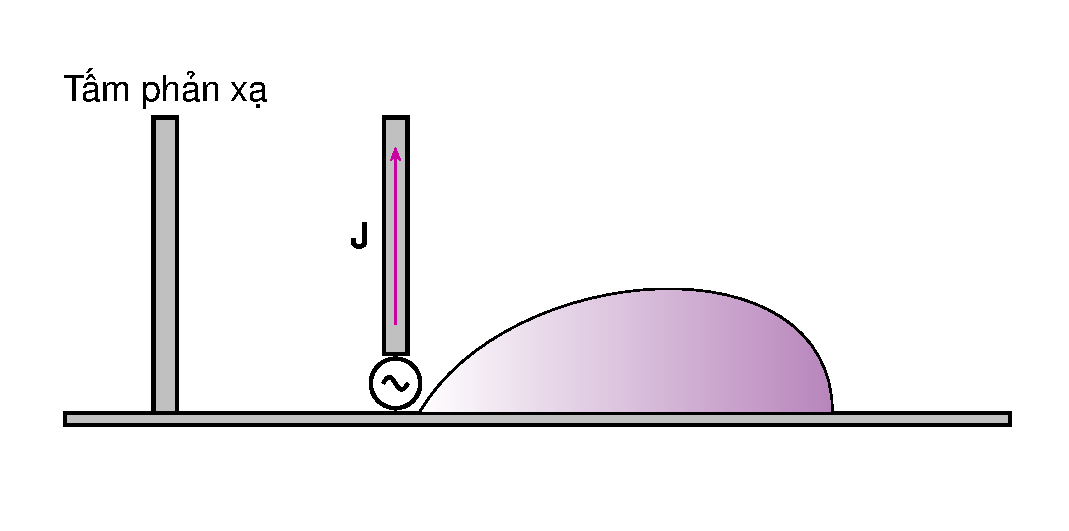
\includegraphics[width=1.0\linewidth]{Figures/Yagi.pdf}
            \caption{Cấu trúc anten Yagi-Uda sử dụng mặt phản xạ trong tái cấu hình búp sóng \cite{10818738} \cite{7001061} \cite{7636946}.}
            \label{fig:Yagi_uda}
        \end{figure}
        \column{0.4\textwidth}
        \begin{figure}
            \centering
            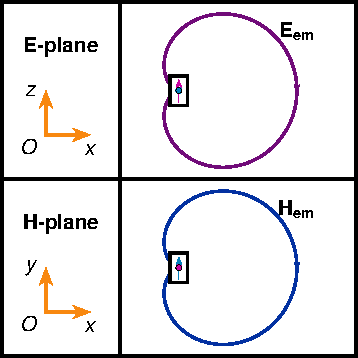
\includegraphics[width=0.75\linewidth]{Figures/MED.pdf}
            \caption{Cấu trúc lưỡng cực điện từ bắt chéo \cite{10621581} \cite{7815297} \cite{8753674} \cite{8421283} \cite{9789208}.}
            \label{fig:MED}
        \end{figure}
    \end{columns}
    \begin{itemize}
        \item Tồn tại: Công nghệ đặc biệt, chi phí sản xuất cao, búp sóng hướng về phía trên.
    \end{itemize}
\end{frame}

